\section{Design Patterns}

\begin{concept}{Grundlagen Design Patterns}
Bewährte Lösungsmuster für wiederkehrende Probleme:
\begin{itemize}
    \item Beschleunigen Entwicklung durch vorgefertigte Lösungen
    \item Verbessern Kommunikation im Team
    \item Bieten Balance zwischen Flexibilität und Komplexität
    \item \textbf{Wichtig:} Design Patterns sind kein Selbstzweck
\end{itemize}
\end{concept}

\subsection{Strukturelle Patterns}

\begin{definition}{Adapter Pattern}
\textbf{Problem:} Inkompatible Schnittstellen integrieren
\begin{itemize}
    \item Objekte mit unterschiedlichen Interfaces sollen zusammenarbeiten
    \item Externe Dienste sollen austauschbar sein
\end{itemize}
\textbf{Lösung:} Adapter-Klasse als Vermittler
%todo: Add adapter pattern diagram
\end{definition}

\begin{definition}{Proxy Pattern}
\textbf{Problem:} Zugriffskontrolle auf Objekte
\begin{itemize}
    \item Verzögertes Laden
    \item Zugriffsbeschränkungen
    \item Netzwerkkommunikation
\end{itemize}
\textbf{Lösung:} Stellvertreterobjekt mit gleichem Interface
\begin{itemize}
    \item \textbf{Remote Proxy:} Für entfernte Objekte
    \item \textbf{Virtual Proxy:} Für spätes Laden
    \item \textbf{Protection Proxy:} Für Zugriffsschutz
\end{itemize}
\end{definition}

\begin{definition}{Decorator Pattern}
\textbf{Problem:} Dynamische Erweiterung von Objekten
\begin{itemize}
    \item Zusätzliche Verantwortlichkeiten
    \item Nur für einzelne Objekte
\end{itemize}
\textbf{Lösung:} Wrapper-Objekt mit gleichem Interface
\end{definition}

\begin{definition}{Composite Pattern}
\textbf{Problem:} Baumstrukturen verwalten
\begin{itemize}
    \item Einheitliche Behandlung
    \item Teil-Ganzes Hierarchie
\end{itemize}
\textbf{Lösung:} Gemeinsames Interface für Container und Inhalt
\end{definition}

\subsection{Verhaltensmuster}

\begin{definition}{Chain of Responsibility Pattern}
\textbf{Problem:} Unklare Zuständigkeit für Anfragen
\begin{itemize}
    \item Mehrere mögliche Handler
    \item Zuständigkeit erst zur Laufzeit klar
\end{itemize}
\textbf{Lösung:} Verkettete Handler-Objekte
\end{definition}

\begin{definition}{Observer Pattern}
\textbf{Problem:} Abhängige Objekte aktualisieren
\begin{itemize}
    \item Lose Kopplung erwünscht
    \item Typ des Empfängers unbekannt
\end{itemize}
\textbf{Lösung:} Observer-Interface für Benachrichtigungen
%todo: Add observer pattern diagram
\end{definition}

\begin{definition}{Strategy Pattern}
\textbf{Problem:} Austauschbare Algorithmen
\begin{itemize}
    \item Verschiedene Implementierungen
    \item Zur Laufzeit wechselbar
\end{itemize}
\textbf{Lösung:} Interface für Algorithmus-Klassen
\end{definition}

\begin{definition}{State Pattern}
\textbf{Problem:} Zustandsabhängiges Verhalten
\begin{itemize}
    \item Verhalten abhängig vom inneren Zustand
    \item Viele bedingte Anweisungen
\end{itemize}
\textbf{Lösung:} Eigene Klassen für verschiedene Zustände
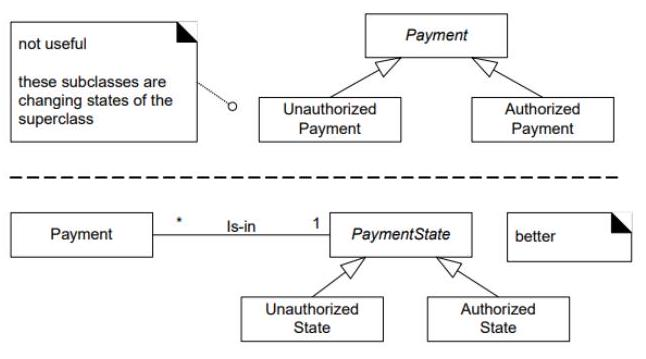
\includegraphics[width=0.7\linewidth]{images/2024_12_29_0d1d7b5551ea1b4b41bdg-07(1)}
\end{definition}

\subsection{Erzeugungsmuster}

\begin{definition}{Factory Method Pattern}
\textbf{Problem:} Flexible Objekterzeugung
\begin{itemize}
    \item Entscheidung über konkrete Klasse zur Laufzeit
    \item Basis für Frameworks/Libraries
\end{itemize}
\textbf{Lösung:} Abstrakte Methode zur Objekterzeugung
\end{definition}

\begin{definition}{Singleton Pattern}
\textbf{Problem:} Genau eine Instanz benötigt
\begin{itemize}
    \item Globaler Zugriffspunkt
    \item Mehrfachinstanzierung verhindern
\end{itemize}
\textbf{Lösung:} Statische Instanz mit privater Erzeugung
\end{definition}

\begin{KR}{Pattern-Analyse für Prüfung}
\textbf{Systematisches Vorgehen:}
\begin{enumerate}
    \item \textbf{Problem identifizieren und analysieren}
    \begin{itemize}
        \item Art des Problems identifizieren
        \item Anforderungen klar definieren
        \item Kontext verstehen
    \end{itemize}
    
    \item \textbf{Pattern auswählen und evaluieren}
    \begin{itemize}
        \item Passende Patterns suchen
        \item Trade-offs abwägen
        \item Kombinationsmöglichkeiten prüfen
    \end{itemize}
    
    \item \textbf{Lösung skizzieren}
    \begin{itemize}
        \item Klassenstruktur entwerfen
        \item Beziehungen definieren
        \item Vor- und Nachteile nennen
    \end{itemize}
\end{enumerate}
\end{KR}

%todo: Add concrete implementation examples for each pattern
%todo: Add comparison matrix of patterns